No aprendizado de máquina, distinguimos três tipos de aprendizado: supervisionado, não supervisionado e de reforço. A distinção geralmente é feita pelo feedback o agente recebe.
A aprendizagem supervisionada é a tarefa de aprender uma função a partir de um conjunto de dados
rotulados. Isso significa que os dados consistem em exemplos de treinamento: as entradas e seus valores de saída desejados. O problema pode ser uma classificação, se a saída for uma
classe, ou um regressão, se a saída for um ou vários valores reais. Em ambos os casos, o feedback é
a saída correta que corresponde à entrada fornecida. Um modelo treinado totalmente supervisionado
serve como uma função que podemos usar para mapear novas entradas. O objetivo é ser capaz de
rotular dados novos corretamente: exemplos que não estavam no conjunto de treinamento. 

Em resumo, o principal objetivo de \textit{Machine Learning} é descobrir padrões a partir do conjunto de dados para que se possa obter \textit{insights} e resolver diversos problemas em campos diferentes. Problemas de aprendizado supervisionado lidam especificamente com dados no formato $(\mathbf{x}^{(i)},y^{(i)})$, em que $y^{(i)}\in\mathbb{R}$ é a saída desejada. Ou seja, a saída também está contida no conjunto de dados.

Em \cite{russel} o principal objetivo do aprendizado supervisionado pode ser definido como:

Dado um \textbf{conjunto de treino} com $N$ pares de entrada-saída 
\begin{gather*}
    \{(\mathbf{x}^{(1)},y^{(1)}),(\mathbf{x}^{(2)},y^{(2)}),...,(\mathbf{x}^{(N)},y^{(N)})\}
\end{gather*}

onde cada $y^{(i)}$ foi gerado por uma função desconhecida $y=f(x)$, devemos descobrir uma função $h$ que se aproxima da real função $f$.

A função $h$ é chamada de \textbf{Hipótese} e está contida em um \textbf{Espaço de Hipóteses} denominado de $\mathcal{H}$ ou seja o espaço contem a classe de funções consideradas por um algoritmo de aprendizagem, que irá escolher a função $h \in \mathcal{H}$ baseado em uma função de erro calculada no \textbf{conjunto de treino} em que a saída $y_i$ é o valor que estamos tentando prever com o nosso modelo.

Em seguida, listamos alguns exemplos clássicos de aprendizado supervisionado: Detecção de fraude em cartões de credito em que $\mathbf{x}^{(i)}$ seriam informações da transação (local, valores, forma de pagamento) e o ${y}^{(i)}$ um indicador booleano se a $i$-th é uma transação fraudulenta ou não. Predição de preços de imóveis em que $\mathbf{x}^{(i)}$ seriam informações do imóvel (local, área do imóvel, quantidade de quartos, ano de construção) e o ${y}^{(i)}$ é o valor do imóvel. Classificação de dígitos manuscritos, onde $\mathbf{x}^{(i)}$ é uma imagem ou a
representação de um número e ${y}^{(i)}$ o número correspondente.

\section{Função Aproximação e Otimização}

A tarefa do aprendizado supervisionado pode ser interpretada como um problema de otimização. Conforme abordado em \cite{hastie}, 
temos o paradigma da \textit{function-fitting}. Do ponto de vista de aprendizado de máquina, vamos assumir que os erros são aditivos e que temos o modelo $Y = f(x) + \epsilon$. A aprendizagem supervisionada tenta aprender $f$ por
exemplo através de um \textit{professor}. 

Observa-se o sistema em estudo, tanto
as entradas quanto as saídas, e monta-se um conjunto de treinamento de observações \simbolo{\mathcal{T}}{Conjunto de treino}$\mathcal{T} =
(\mathbf{x}^{(i)},{y}^{(i)}), i = 1, . . . , N$ . Os valores de entrada observados para o sistema $\mathbf{x}^{(i)}$ também são alimentados em um sistema artificial, conhecido como um algoritmo de aprendizagem, que também produz saídas $\hat{f}(x^{(i)})$ em resposta. O algoritmo de aprendizado tem a propriedade de poder modificar sua relação de entrada/saída $\hat{f}$ em resposta às diferenças ${y}^{(i)}-\hat{f}(x^{(i)})$ entre as saídas originais e geradas. Esse processo é conhecido como \textit{aprendizado por exemplo}. Após a conclusão do processo de aprendizagem, o objetivo final é que as saídas artificiais e as saídas reais estejam próximas o suficiente para o modelo consiga generalizar para todos os conjuntos de entradas.

As diferentes funções $\hat{f}$ podem ser estimadas a partir de diferentes modelos em que a hipótese escolhida se aproximará da verdadeira função $f$. Alguns exemplos são estimativa por máxima verossimilhança, o método dos mínimos quadrados, expansões lineares e transformação \textit{sigmoid}.

Para estimar os parâmetros dessas aproximações, os algoritmos de aprendizado geralmente realizam uma otimização sobre uma \textit{função de perda} \cite{kuhn} que depende do aproximador escolhido.

\section{Viés-Variância \textit{Tradeoff}}
O objetivo dos modelos de aprendizado de máquina é estimar a função que melhor ajusta aos dados de entrada para obter previsões corretas de forma generalizada. A melhor maneira de medir e otimizar o desempenho do modelo é levar em consideração o viés e a variância.

O problema básico de aprendizado supervisionado geralmente consiste em dois conjuntos de dados: \textbf{conjunto de treinamento} e
o \textbf{conjunto de teste}. Um modelo é treinado usando dados do conjunto de treinamento, resultando em um modelo $\hat{f}$, então este modelo prevê os dados no conjunto de teste, e com o previsto $\hat{y}^{(i)}$ é possível estimar o erro de previsão do modelo.

Se estivermos em uma situação com bastante volume de dados, a melhor abordagem é dividir aleatoriamente o conjunto de dados em três partes: um conjunto de treinamento, um conjunto de validação e um conjunto de teste. O conjunto de treinamento é usado para ajustar os modelos, a validação é usado para estimar o erro de previsão para a seleção do modelo, o conjunto de teste é utilizado para avaliação do erro do modelo final escolhido.

Idealmente, o conjunto de teste deve ser mantido separado dos outros conjuntos e ser utilizado apenas no final da análise de dados. Suponha que usamos o conjunto de teste repetidamente, escolhendo o modelo com o menor erro desse conjunto, então o  erro definitivo do modelo final escolhido irá subestimar o verdadeiro erro de teste, às vezes substancialmente.
É difícil dar uma regra geral sobre como escolher o número de
observações em cada uma das três partes, pois isso depende do conjunto de dados em si, quantidade de ruído e o tamanho da amostra de treinamento, porém uma divisão típica pode
ser 50\% para treinamento e 25\% cada para validação e teste:

\begin{figure}[htb]
 \caption{Divisão de Treino, Validação e Teste}
 \label{fig:treino_test_split}
 \centering
 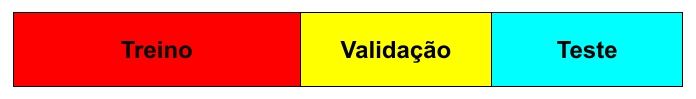
\includegraphics[scale=0.4]{images/treino_teste_split.png}
\end{figure}


O \textit{tradeoff} de viés-variância \cite{hastie} na modelagem preditiva afeta a capacidade de um método de aprendizagem para generalizar. Alta variância indica que o modelo ajusta o ruído aleatório no conjunto de treinamento, o que geralmente resulta em baixo poder de generalização, causando o \textbf{overfitting}. Por outro lado, um modelo com viés alto tem uma diferença muito baixa no erro de previsão entre o conjunto de treinamento e conjunto de teste, mas geralmente tem desempenho ruim causando o \textbf{underfitting}. 

No treinamento e avaliação do modelo, é importante verificar o desempenho da generalização, e isso geralmente é feito usando o conjunto de teste. No processo de avaliação, o \textbf{overfitting} e o \textbf{underfitting} podem ser detectados comparando o erro de previsão no conjunto de treinamento e teste.

A Figura \ref{fig:bias_variance_comp} ilustra uma questão importante na avaliação da capacidade de generalização do modelo. Considere primeiro o caso de um quantitativo ou intervalo resposta de escala. Temos uma variável de resposta $Y$ , um vetor de entradas $\mathbf{X}$ e um modelo de predição $\hat{f}(X)$ que foi estimado a partir de um conjunto de treinamento $\mathcal{T}$ . 

A função para medição do erro entre $Y$ e $\hat{f}(X)$ é denotada por $L(Y,\hat{f}(X))$. Ainda neste Capítulo serão abordadas demais formas para medir o desempenho, mas algumas escolhas típicas para esse erro são:
\begin{equation}
  L(Y,\hat{f}(X)) =
    \begin{cases}
      {(Y - \hat{f}(X))}^2 & \text{erro quadrático}\\
      |Y - \hat{f}(X)| & \text{erro absoluto}
    \end{cases}       
\end{equation}

\begin{figure}[htb]
 \caption{Comportamento das amostra de teste e treino conforme a complexidade do modelo é variada. As curvas em azul claro mostram o erro $\overline{err}$ de treinamento, enquanto o
curvas vermelhas claras mostram o erro de teste condicional $Err_{\mathcal{T}}$ para 100 conjuntos de treinamento de tamanho 50 cada, à medida que a complexidade do modelo aumenta. As curvas sólidas mostram o  erro de teste esperado $Err$ e o erro de treinamento esperado $E[\overline{err}]$ \cite{hastie}
}
 \label{fig:bias_variance_comp}
 \centering
 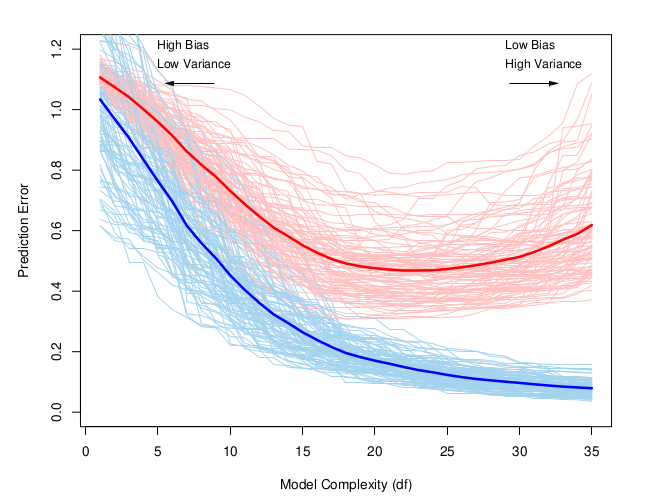
\includegraphics[scale=0.5]{images/bias_viariance.png}
\end{figure}

O erro do teste em uma amostra independente é dado por:

\begin{equation}
    Err_{\mathcal{T}} = E[L(Y,\hat{f}(X))|\mathcal{T}]
\end{equation}

Em que tanto $X$ quanto $Y$ são amostras aleatórias da população. Neste caso, o conjunto de treino $\mathcal{T}$ é fixo e o erro do conjunto de teste é referente a este conjunto de treino fixo $\mathcal{T}$. Podemos escrever esse erro como:
\begin{equation}
    Err = E[L(Y,\hat{f}(X))] = Err_{\mathcal{T}}
\end{equation}

O objetivo é estimar o $Err_{\mathcal{T}}$.

\section{Problema de Classificação}
Conforme foi abordado no Capítulo \ref{chapter:introducao}, quando os valores de $f$ pertencem a um conjunto finito temos um problema de classificação e especialmente quando o valor de $f$ assume apenas dois possíveis valores denotamos de \textbf{classificação binária}.
\begin{figure}[htb]
 \caption{Exemplo de limite de decisão para um classificador binário \cite{hastie}.}
 \label{fig:clas_ex}
 \centering
 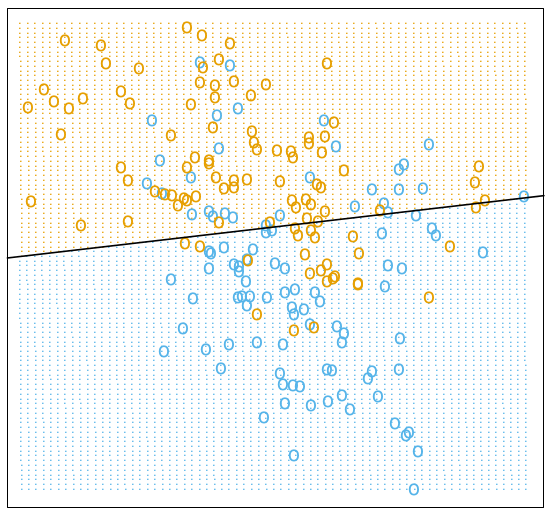
\includegraphics[scale=0.4]{images/classificacao_hastie_ex.png}
\end{figure}

O exemplo de detecção de fraude no cartão de cŕedito que foi abordado no começo deste Capítulo é um problema de classificação bińaria.

\section{Métricas de Avaliação de Performance}
Existem diversas métricas para avaliar a performance de modelos de classificação. Neste estudo as métricas abordadas serão a \textit{AUC}, que é um acrônimo da área em baixo da curva característica de operação do receptor, \textit{Logloss}, que é a perda logarítmica, e o \textit{KS}, que é o Teste Kolmogorov-Smirnov. Um breve resumo de cada métrica:

\begin{itemize}
    \item \textbf{AUC:} é amplamente utilizado em pesquisas, e é uma boa métrica insensível ao desequilíbrio de classes, tendo um valor limitado entre 0.5 e 1.
    \item \textbf{Logloss:} \textit{logloss} é a função direta otimizada nos experimentos, ou seja, as etapas de aumento de gradiente estão tentando reduzir a perda logarítmica em cada etapa. O \textit{logloss} leva em conta a incerteza da previsão e quanto o rótulo real difere dela, tendo seu valor limitado a $]\infty,0]$
    \item \textbf{KS:} o teste Kolgomorov-Smirnov (KS) busca avaliar a distância entre uma distribuição conhecida e uma distribuição que foi observada empiricamente. A hipótese nula do KS é que a amostra segue a mesma distribuição que a normal, tendo o valor limitado entre 0 e 1.
\end{itemize}

\subsection{AUC}

A curva característica de operação do receptor é uma curva de probabilidade que mede a previsão de um classificador binário dado um \textit{threshold}. Os resultados de uma classificação binária podem ser resumidos em uma matriz de confusão, ilustrada na Tabela \ref{tabela:matriz_conf}.Os Verdadeiro-positivo (VP), Falso-positivo (FP), Falso-negativo (FN) e Verdadeiro-negativo (VN) são calculados dispondo todos os dados na matriz, dependendo da classe prevista e da classe real de cada ponto no conjunto de dados.

\begin{table}[htb]
\centering
\caption{Matriz de confusão para o problema de classificação binária.}
\label{tabela:matriz_conf}
\begin{tabular}{|p{3cm}|p{5cm}|p{5cm}|} 
 \hline
\textbf{Resultado} & \multicolumn{2}{c|}{\textbf{Classe Real}} \\
  \hline
  \textbf{Classe Predita} & \textbf{Positivo} & \textbf{Negativo} \\
  \hline
  \textbf{Positivo} & Verdadeiro-positivo (VP) & Falso-positivo (FP) \\
  \hline
  \textbf{Negativo} & Falso-negativo (FN) & Verdadeiro-negativo(VN) \\
  \hline
\end{tabular}
\end{table}

\begin{figure}[htb]
 \caption{Uma ilustração da ocorrência de eventos positivos e negativos
quando ordenado pela variável contínua $y$ \cite{BROWN200624}.}
 \label{fig:roc_brown}
 \centering
 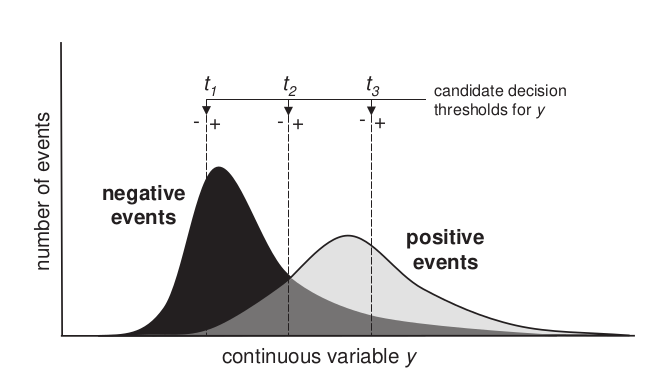
\includegraphics[scale=0.5]{images/roc_threshold.png}
\end{figure}

Conforme abordado em \cite{BROWN200624}, \cite{FAWCETT2006861} e \cite{kuhn} a curva característica do operador (ROC) é calculada pelo gráfico de \textit{Taxa de Verdadeiros Positivos (TVP)}, ou Sensibilidade, versus \textit{Taxa de Falso Positivos (TFP)}, ou Especificidade, onde $\mathcal{T}$ é o \textit{threshold}.

\begin{gather*}
    Roc_{y}(\mathcal{T}) = TVP_{\mathcal{T}} = \frac{VP_{\mathcal{T}}}{VP_{\mathcal{T}} + FN_{\mathcal{T}}} \\
    Roc_{x}(\mathcal{T}) = TFP_{\mathcal{T}} = \frac{FP_{\mathcal{T}}}{FP_{\mathcal{T}} + VN_{\mathcal{T}}}
\end{gather*}

\begin{figure}[H]
 \caption{Curva ROC de um classificador \cite{kuhn}, dois pontos estão em destaques para mostrar diferentes valores de \textit{Especificidade} e \textit{Sensibilidade}}
 \label{fig:roc_kuhn}
 \centering
 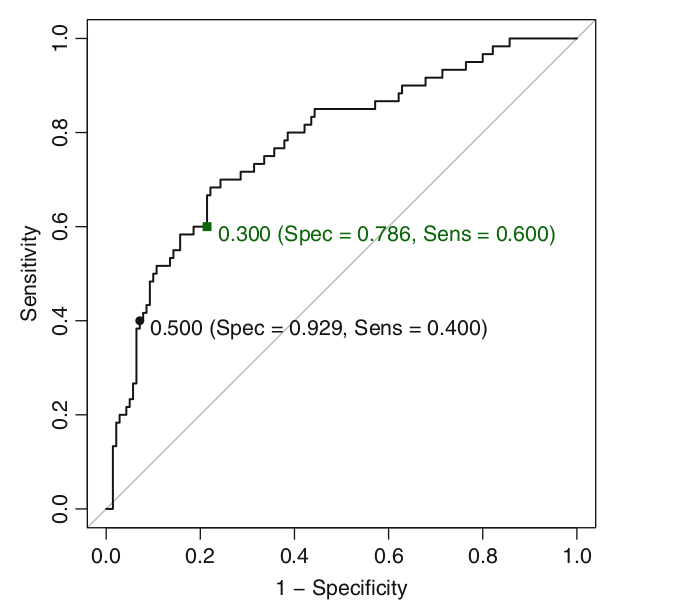
\includegraphics[scale=0.4]{images/roc_kuhn.png}
\end{figure}

Todas as métricas dependem do \textit{threshold} $\mathcal{T}$. A \textbf{AUC} é definida como a área em baixo da curva ROC e fornece uma medida agregada do desempenho do classificador em relação a todos os \textit{threshold} possíveis. O valor é entre 0.5 (pior performance) e 1 (performance perfeita).

Abaixo temos os algoritmos para a geração dos pontos da curva \textbf{ROC} e do cálculo da \textbf{AUC} \cite{FAWCETT2006861}.

\begin{algorithm}[H]
\caption{Algoritmo de geração de curva ROC}\label{algoritmo:roc}
\label{algo:roc}
\textbf{Input:} $L$, o conjunto de exemplos de teste; $f(i)$, o modelo probabilístico
dos classificadores que estimam que o exemplo $i$ é positivo, $P$ e $N$, o
número de exemplos positivos e negativos.\\
\textbf{Output:} $R$, uma lista de pontos ROC aumentando pela taxa FP. \\
\textbf{Requer:} $P>0$ e $N>0$. \\
\begin{algorithmic}[1]
\State $L_{sorted}$ \Comment{$L$ ordenada pelos valores decrescentes de $f$}
\State $FP$ $\leftarrow$ $VP$ $\leftarrow$ $0$ 
\State $R$ $\leftarrow$ [] 
\State $f_{prev}$ $\leftarrow -\infty$ 
\State $i$ $\leftarrow$ $1$
\While{$i\leq |L_{sorted}|$} 
\If{$f(i) \neq f_{prev}$}
\State push $(\frac{FP}{N},\frac{VP}{P})$ onto $R$
\State $f_{prev} \leftarrow f(i)$
\EndIf
\If{$L_{sorted}[i]$ for positivo}
\State $VP \leftarrow VP + 1$
\Else
\State $FP \leftarrow FP + 1$
\EndIf
\State $i \leftarrow i + 1$
\EndWhile
\State push $(\frac{FP}{N},\frac{VP}{P})$ onto $R$
\end{algorithmic}
\end{algorithm}

\begin{algorithm}[H]
\caption{Algoritmo para calcular a área em baixo da curva ROC}\label{algoritmo:auc}
\label{algo:auc}
\textbf{Input:} $L$, o conjunto de exemplos de teste; $f(i)$, o modelo probabilístico
dos classificadores que estimam que o exemplo $i$ é positivo, $P$ e $N$, o
número de exemplos positivos e negativos.\\
\textbf{Output:} $A$, a área em baixo da curva ROC. \\
\textbf{Requer:} $P>0$ e $N>0$. \\
\begin{algorithmic}[1]
\State $L_{sorted}$ \Comment{$L$ ordenada pelos valores decrescentes de $f$}
\State $FP$ $\leftarrow$ $VP$ $\leftarrow$ $0$ 
\State $FP_{prev}$ $\leftarrow$ $VP_{prev}$ $\leftarrow$ $0$ 
\State $A$ $\leftarrow$ $0$
\State $f_{prev}$ $\leftarrow -\infty$ 
\State $i$ $\leftarrow$ $1$
\While{$i\leq |L_{sorted}|$} 
\If{$f(i) \neq f_{prev}$}
\State $A \leftarrow A +$  AREA\_TRAPEZIO($FP,FP_{prev},VP,VP_{prev}$)
\State $f_{prev} \leftarrow f(i)$
\State $FP_{prev} \leftarrow FP$
\State $VP_{prev} \leftarrow VP$
\EndIf
\State $i \leftarrow i + 1$
\If{$i$ for positivo}
\State $VP \leftarrow VP + 1$
\Else
\State $FP \leftarrow FP + 1$
\EndIf
\State $i \leftarrow i + 1$
\EndWhile
\State $A \leftarrow A +$  AREA\_TRAPEZIO($N,FP_{prev},N,VP_{prev}$)
\State $A \leftarrow  \frac{A}{P \times N}$
\Function {AREA\_TRAPEZIO}{$X1,X2,Y1,Y2$}
\State Base $\leftarrow |X1 - X2|$
\State Altura $\leftarrow \frac{Y1+Y2}{2}$
\State \Return Base $\times$ Altura
\EndFunction
\end{algorithmic}
\end{algorithm}

\subsection{Logloss}
Perda Logarítmica ou \textbf{Logloss} é uma função que mede a precisão de um classificador penalizando erros com base na incerteza na previsão, ou seja, verifica se as probabilidades emitidas pelo modelo estão alinhadas com a proporção real de ocorrências do alvo \cite{DBLP:journals/corr/Vovk15}. Nessa métrica, quanto menor o valor melhor: o 0 é a predição perfeita. Conforme veremos no Capítulo \ref{chapter:algoritmos-boosting}, essa é a função de perda que é normalmente otimizada pelos algorítimos de boosting.

A equação da \textit{logloss} para classificadores binários é dada por:
\begin{equation}
    Logloss = -\frac{1}{N}\sum_{i=1}^n[y^{(i)}\log \hat{y}^{(i)} + (1-y^{(i)})\log(1-\hat{y}^{(i)})]
\end{equation}

O gráfico abaixo mostra a faixa de possíveis valores de perda dada uma observação verdadeira (\textit{target} = 1). À medida que a probabilidade prevista se aproxima de 1, a perda de logarítmica diminui lentamente enquanto que à medida que a probabilidade prevista diminui, a perda de logarítmica aumenta rapidamente. A perda de logarítmica penaliza ambos os tipos de erros, mas especialmente aquelas previsões que não são confiáveis.

\begin{figure}[H]
 \caption{\textit{Logloss} em função das predições de uma observação \cite{mlcheat:log}}.
 \label{fig:log_loss_gra}
 \centering
 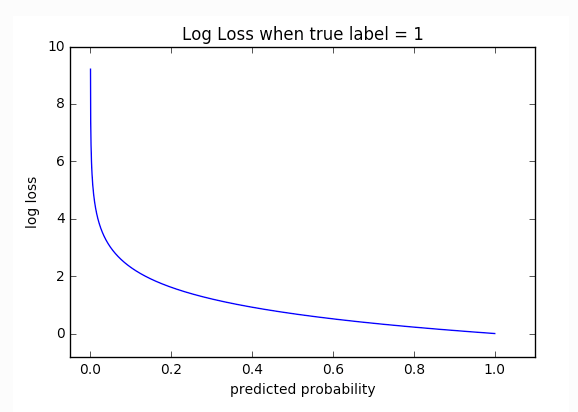
\includegraphics[scale=0.5]{images/logloss_grap.png}
\end{figure}


\subsection{Teste de Kolmogorov-Smirnov}
O Teste de Kolmogorov-Smirnov \cite{kolmogorov,smirnov} também é conhecido como teste de KS ou teste K-S. É um teste de aderência: verifica o grau de concordância entre a distribuição de um conjunto de valores (por exemplo, os escores observados pelo modelo) e alguma distribuição teórica. Esse teste pode ser usado para verificar se os dados seguem, por exemplo, a distribuição normal. A distribuição de frequência acumulada é comparada com a distribuição de frequência observada. A distribuição teórica representa o que seria esperado sobre $H_0$\simbolo{H_0}{Hipótese Nula}, hipótese nula. É determinado o ponto em que as duas distribuições, teórica e observada, tem a maior diferença. \cite{nonparametric}. 

Seja $F_0(X)$ uma função de distribuição de frequências relativas acumuladas, a distribuição teórica sob $H_0$, pra qualquer valor de $X$, o valor de $F_0(X)$  ́e a proporção de casos esperados com escores menores ou iguais a $X$.

Seja $\hat{F}_n$ a distribuição de frequências relativas acumuladas observada de uma amostra aleatória de $N$ observações, se $X_i$ é um escore qualquer, então $\hat{F}(X_i) = \frac{F_i}{N}$ em que $F_i$ é o número de observações menores ou iguais a $X_i$. As hipóteses do testes são $H_0$: a amostra vem de uma distribuição teórica específica (por exemplo a distribuição normal), ou $H_1$\simbolo{H_1}{Hipótese Alternativa}, a amostra não provém de uma distribuição teórica especifica.

O teste espera que quando $H_0$ é verdadeira as diferenças entre $\hat{F}(X_i)$ e $F_0(X_i)$ sejam pequenas e estando dentro do limite dos erros aleatórios. O maior dos desvios é usado, chamado de desvio máximo
\begin{gather}
    D = \max(F_0(X_i)-\hat{F}(X_i))
\end{gather}

A hipótese é verificada através do teste \textit{p-valor} com $D = \max(F_0(X_i)-\hat{F}(X_i)) < D_{(N,\alpha)}$, onde $D_{(N,\alpha)}$ é um valor tabelado . Nesse caso, não rejeitamos $H_0$ e caso no contrario, $D = \max(F_0(X_i)-\hat{F}(X_i)) > D_{(N,\alpha)}$, rejeitamos $H_0$. \cite{bussab}.
\begin{figure}[H]
 \caption{KS: diferença entre as funções de distribuição \cite{ashwin}.}
 \label{fig:roc_kuhn}
 \centering
 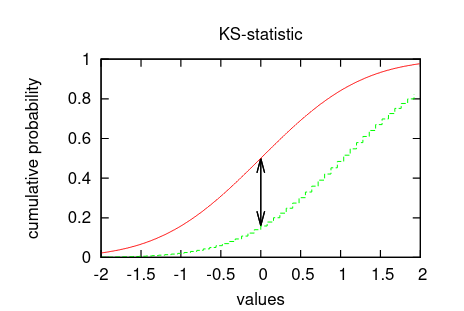
\includegraphics[scale=0.6]{images/ks_statis.png}
\end{figure}

Para o problema de classificação binária o KS pode ser calculado a partir da \textit{Taxa de Verdadeiros Positivos (TVP)} e da \textit{Taxa de Falso Positivos (TFP)}.
\begin{equation}
    KS = \max(TVP - TFP)
\end{equation}
Abaixo temos o algoritmo para o cálculo do KS de \textit{OneSample} \cite{ashwin}.
\begin{algorithm}[H]
\caption{KS: OneSample($Q,n,F$)}\label{algoritmo:ks}
\textbf{Input:} Quantil $Q$, número de dados $n$ e a função de distribuição $F$. \\
\textbf{Output:} $\hat{D}$, o valor estimado de KS. \\
\begin{algorithmic}[1]
\State Seja $X_{i1} \leq X_{i2} \leq ... \leq X_{ik}$ valores em $Q$
\State $\hat{D}$ $\leftarrow$ $0$ 
\If{cada $x\in (X_{i1},...,X_{ik})$} 
\State $j = \max(p | X_{ip}\leq x)$
\State seja $\hat{i_j}$ aproximadamente o índice de $X_{ij}$
\State $\hat{E}_x = | \frac{\hat{i_j}}{n - F(x)}$
\State $\hat{D} = \max(\hat{D},\hat{E}_x)$
\EndIf
\State \Return $\hat{D}$
\end{algorithmic}
\end{algorithm}


\section{Hiperparâmetros e Model Tuning}
Conforme vimos no Capítulo \ref{chapter:introducao} e será abordado nos próximos Capítulos, muitos modelos de aprendizado supervisionado possuem parâmetros que não podem ser diretamente estimados pelo conjunto de treino. Muitos desses parâmetros afetam a qualidade do modelo prever resultados a partir de novos dados de entrada. Esses parâmetros são intrínsecos dos modelos pois representam características deles, como o número de interações, o termo de regularização, o tamanho da árvore e etc. Esses parâmetros precisam ser escolhidos antes do início do processo de aprendizado do algoritmo, e são denominados de hiperparâmetros e o processo de escolha desses parâmetros visando a melhoria da performance do modelo é conhecido como \textit{tuning hyperparameter} \cite{ian,kuhn,tuning:artigo,hyper:op:theory,grid:book,neural:op}.

Para lidar com os hiperparâmetros existem duas abordagens: escolher eles manualmente 
ou utilizar um algoritmo para escolher automaticamente. A escolha manual requer o entendimento profundo da influência dos hiperparâmetros e como os modelos de aprendizagem de máquina alcançam uma boa generalização. Geralmente consiste em retreinar o modelo varias vezes com apenas a alteração dos hiperparâmetros e validando as performance de cada treino. Por outro lado, a seleção automática de hiperparâmetros reduz a necessidade de entender a fundo sua influência, porém requer um maior poder de processamento computacional.

Idealmente, um algoritmo de aprendizagem usaria apenas o conjunto de dados e geraria uma função, não exigindo ajuste manual de hiperparâmetros. A popularidade de vários  algoritmos como regressão logística e SVMs decorre, em parte, de sua capacidade de trazer resultados satisfatórios com apenas um ou dois hiperparâmetros ajustados. As redes neurais podem também funcionar bem com apenas um pequeno número de hiperparâmetros ajustados, mas muitas vezes se beneficiam significativamente do ajuste de quarenta ou mais hiperparâmetros. O ajuste de hiperparâmetros pode funcionar muito bem quando o usuário tem um bom ponto de partida, como aquele determinado por outros que trabalharam no mesmo tipo de aplicativo e arquitetura, ou quando o usuário tem meses ou anos de experiência em explorar valores de hiperparâmetros para redes neurais aplicadas a tarefas semelhantes. No entanto, para muitas aplicações, esses pontos de partida não estão disponíveis. Nesses casos, algoritmos automatizados podem encontrar valores úteis dos hiperparâmetros\cite{tree:tunning}.

Estamos tentando encontrar um valor dos hiperparâmetros que otimize uma função objetivo, como o erro de validação, às vezes sob restrições. Portanto, é possível, em princípio, desenvolver algoritmos de otimização de hiperparâmetros que envolvam um algoritmo de aprendizado de máquina e escolha seus hiperparâmetros, ocultando do usuário do algoritmo de aprendizado o ajuste dos hiperparâmetros. Infelizmente, a otimização de hiperparâmetros dos algoritmos geralmente têm seus próprios hiperparâmetros, como o intervalo de valores que deve ser explorado para cada um dos hiperparâmetros do algoritmo de aprendizado de máquina. No entanto, esses hiperparâmetros secundários são geralmente mais fáceis de escolher, no sentido de que um desempenho aceitável pode ser alcançado em uma ampla gama de tarefas usando os mesmos hiperparâmetros secundários para todas as tarefas.

O processo de tunar os hiperparâmetros geralmente é tratado como uma problema de otimização caixa-preta. De maneira formal, podemos definir o problema como:
Seja:
\begin{gather*}
    \simbolo{\mathcal{H}}{Espaço de Hiperparâmetro} \mathcal{H} = \mathcal{H}_1 \times \mathcal{H}_2 \times ... \times \mathcal{H}_k
\end{gather*}
O espaço dos hiperparâmetros e um algoritmo $a\in \mathcal{A}$ em que $\mathcal{A}$ é um conjunto de algoritmos de aprendizado de máquina. Cada $\mathcal{H}_i$ representa um conjunto de possíveis valores para o hiperparâmetro $i^{th}$ de $a(i\in\{1,...,k\})$. Seja $\mathcal{D}$ um conjunto de dados em que $D\in \mathcal{D}$ é um conjunto de dados de $\mathcal{D}$. A função $f:\mathcal{A}\times \mathcal{D} \times \mathcal{H}\rightarrow \mathbb{R}$ calcula a performance do modelo pelo algoritmo $a\in \mathcal{A}$ no conjunto de dados $D\in \mathcal{D}$ dado a configuração de hiperparâmetros $h=(h_1,h_2,...,h_k)\in\mathcal{H}$.

Dado $a\in \mathcal{A},\mathcal{H}$ e $D\in \mathcal{D}$ o objetivo da tunar os hiperparâmetros é encontrar $h^*=(h_1^*,h_2^*,...,h_k^*)$ tal que :
\begin{equation}
    h^* = {arg\max}_{h\in\mathcal{H}} f(a,D,h)
\end{equation}

Existem diversas técnicas que buscam otimizar os hiperparâmetros, irei exemplificar algumas, para um estudo mais completo consultar \cite{hyper:op:theory,grid:book,neural:op}.
\subsection{Grid Search}
É um dos métodos mais comuns utilizado para explorar o espaço de configuração de hiperparâmetros é o Grid Search. Ele pode ser considerado uma busca exaustiva ou um método de força bruta que avalia todas as combinações de hiperparâmetros dadas à uma 'grade' de configurações. O Grid Search funciona avaliando o produto cartesiano de um conjunto finito de valores especificado pelo usuário, ele não pode explorar as regiões de bom desempenho por si só. Portanto, para identificar os ótimos globais, o seguinte procedimento precisa ser realizado manualmente \cite{grid:article,grid:book,grid:random:2}.

\begin{enumerate}
    \item Comece com um grande espaço de busca e tamanho de passo definidos. 
    \item Restrinja o espaço de pesquisa e o tamanho do passo com base nos resultados anteriores de hiperparâmetros. 
    \item Repita a etapa 2 várias vezes até que um ótimo seja alcançado.
\end{enumerate}

O Grid Search pode ser facilmente implementado e paralelizado. No entanto, a sua principal desvantagem é a sua ineficiência para alta dimensionalidade de espaço de configuração de hiperparâmetros, já que o número de interações aumenta exponencialmente à medida que o número de hiperparâmetros cresce, esse crescimento exponencial é conhecido como a maldição da dimensionalidade. Para Grid Search, assumindo que existem $k$ parâmetros, e cada um deles com $n$ valores distintos, sua complexidade computacional é de $\mathcal{O}(n^k)$. Logo, o Grid Search só se torna um algorítimo eficiente quando o espaço de configurações de hiperparâmetros é pequeno.

\subsection{Random Search}
Para superar certas limitações do Grid Search, o Random Search foi
proposto \cite{randoms,grid:book,grid:random:2}. Ele é bem semelhante ao Grid Search mas ao invés de testar todos os valores no espaço de configuração ele seleciona aleatoriamente um número pré definido de amostrar entre os limites superior e inferior e em seguida treina essas amostras. Ele é capaz de explorar um espaço de busca maior que o Grid Search, ele é facilmente paralelizado pois cada avaliação é independente. Como o número total de avaliações no Random Search é
definido para um valor fixo $n$ antes do início do processo de otimização, a complexidade computacional  é $\mathcal{O(n)}$. Além disso, Random Search pode detectar o ótimo global ou um ótimo local quando fornecido poder computacional o suficiente.

A principal limitação desses dois métodos é que cada avaliação é independente da avaliação anterior, ou seja, eles perdem muito tempo avaliando combinações ruins de hiperparâmetros.


\subsection{Otimização Bayesiana}
Para resolver a limitação do Random Search e Grid Search, temos os algoritmos de otimização Bayesiana, que são algorítimos interativos que determinam o ponto de avaliação futura com base no resultado obtido na interação passada. Para determinar a próxima configuração de hiperparâmetro, o algoritmo usa dois componentes principais: um modelo substituto e uma função de aquisição (ou seleção).
O modelo substituto (processo gaussiano) visa atender a todos os pontos observados na função objetivo. Depois de obter a distribuição posterior de funções que melhor descreve a função que você deseja otimizar a função de aquisição determina o uso de diferentes pontos para equilibrar o trade-off entre \textit{exploration} e \textit{exploitation} \cite{grid:book,opt:bay}.
\textit{Exploration} consiste em amostrar as instâncias nas áreas que não
foram amostrados, enquanto \textit{exploitation} é para amostrar nas atuais regiões promissoras onde o ótimo global é mais provável, com base na distribuição posterior. Os modelos de otimização Bayesiana equilibram ambos os processos para detectar as atuais regiões mais prováveis e evitar a perda de melhores configurações nas áreas inexploradas.
Os procedimentos do algoritmo são:

\begin{enumerate}
    \item Construir um modelo substituto probabilístico da função objetivo. 
    \item Detecte os valores ideais de hiperparâmetros no
modelo substituto.
\item Aplique esses valores de hiperparâmetros à função objetiva para avaliação.
\item Atualize o modelo substituto com novos resultados.
\item Repita as etapas 2 a 4 até que o número máximo de iterações seja
alcançado.
\end{enumerate}

Assim, o algoritmo de otimização Bayesiana funciona atualizando o modelo substituto após cada
avaliação na função objetivo. A otimização Bayesiana é mais eficiente que Grid Search e o Random Search, pois pode detectar a combinação ideal de hiperparâmetros analisando os valores testados anteriormente.


\section{Árvore de Decisão}
A maioria dos algoritmos de boosting utilizam árvores de decisão como aprendizes básicos. 
Uma árvore é uma coleção de elementos chamados de nós, dentre os quais um é distinguido como uma raiz, juntamente com uma relação de “paternidade” que impõe uma estrutura hierárquica sobre os nós.

Uma Árvore de Decisão é:
\begin{itemize}
    \item um nó folha (ou nó resposta) que contém o nome de uma classe ou o símbolo nulo (nulo indica que não é possível atribuir nenhuma classe ao nó por não haver nenhum exemplo que corresponda a esse nó)
\item um nó interno (ou nó de decisão) que contém o nome de um atributo; para cada possível valor do atributo, corresponde um ramo para uma outra árvore de decisão.
\end{itemize}
E temos uma estrutura típica para uma árvore de decisão:
\begin{itemize}
    \item Nós internos são rotulados com atributos.
    \item Folhas são rotuladas com classes
    \item Ramos são rotulados com valores (atributos categóricos) ou com intervalos (atributos numéricos).
\end{itemize}
Uma árvore de decisão é uma representação de uma função que mapeia um vetor de valores de atributos para um único valor de saída, uma "decisão". Uma árvore de decisão chega à sua decisão realizando uma sequencia de testes, começando na raiz e seguindo o ramo apropriado até que uma folha seja alcançada. Cada nó interno na árvore corresponde a um teste do valor de uma das entradas atributos, os ramos do nó são rotulados com os possíveis valores do atributo, e os nós folha especificam qual valor deve ser retornado pela função. O processo de aprendizado de uma árvore de decisão é chamado de indução da árvore de decisão. A ideia do algoritmo é escolher as divisões internas da árvore que melhor explicam os dados e é, em si, uma pequena árvore. Na figura \ref{fig:ex:arvore} temos um exemplo de uma aŕvore de decisão treinada \cite{russel}.

\begin{figure}[H]
 \caption{Exemplo de uma árvore de decisão \cite{russel}.}
 \label{fig:ex:arvore}
 \centering
 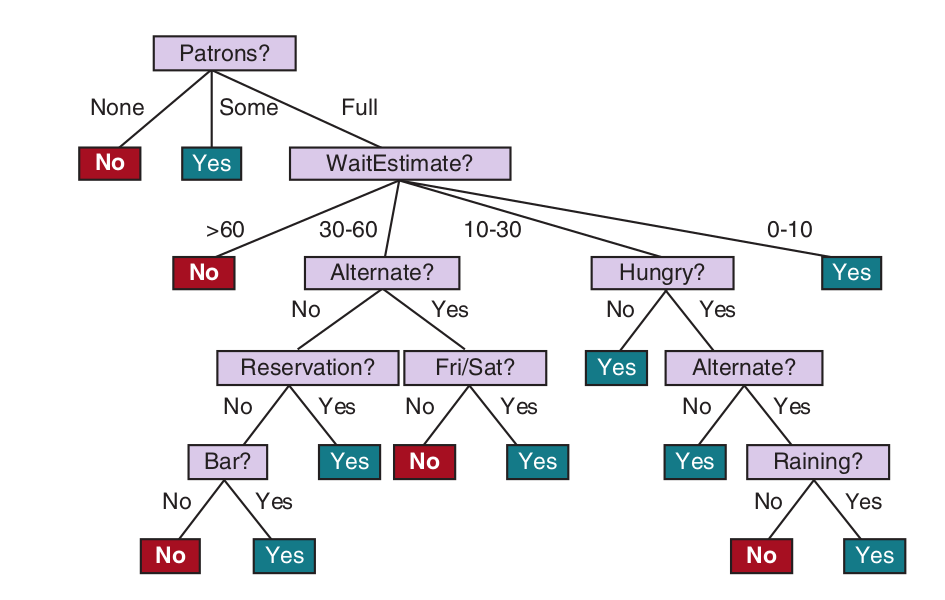
\includegraphics[scale=0.4]{images/exemplo_arvore.png}
\end{figure}

O processo de aprendizado das árvores de classificação consiste em várias iterações para escolher as melhores divisões a partir dos dados de treinamento fornecidos, de acordo com critérios. Os critérios mais comuns de otimização são
geralmente advindos da Teoria da Informação, como o Índice de Gini e a Entropia Cruzada.
O índice de Gini, $G(D)$ no nó $S$ na árvore de decisão pode ser definido como:
\begin{gather*}
    G(S) = 1 - \sum_{i=1}^cp_i^2
\end{gather*}
O algoritmo \ref{algoritmo:arvore} mostra o pseudo código para o algoritmo de árvore de decisão \cite{tree:algor:risk}.
\begin{algorithm}[H]
\caption{Árvore de decisão.\label{algoritmo:arvore}}
\textbf{Input:} Conjunto de treino $D=\mathbf{x}^{(1)},y^{(1)}),(\mathbf{x}^{(2)},y^{(2)}),(\mathbf{x}^{(i)},y^{(j)}$. Atributos $A=(a_1,a_2,..._a_k)$. Método de seleção do atributo: Utilizaremos o \textit{Gain Ratio} para separar o atributo e o sub conjunto de dados $GR(D,a)=\frac{G(D,a)}{Entropia(a)}$, em que $Entropia(D)= \sum_{i=1}^c-p_ilog_2p_i$ e o $G(D,a)=Entropia(D) - \sum_{v\in Values(a)}^{} \frac{|D_v|}{D}Entropia(D_v)$, em que $Values(a)$ são todos os possíveis valores do atributo $a$ e $D_v$ é um sub conjunto do nosso conjunto de dados $D$ que para cada atributo tem o valor $v$.\\
\textbf{Output:} Árvore de decisão. \\
\begin{algorithmic}[1]
\State criar o nó $N$
\If{as amostras de $D$ estão na mesma classe $C$} 
\State \Return $N$ como nó folha rotulado com a classe $C$
\EndIf
\If{$A \neq 0 $ ou o valor do atributo em $D$ são o mesmo}
\State \Return $N$ como nó folha rotulado com a classe em $D$
\EndIf
\State ache o melhor atributo $a\in A$ utilizando um método de seleção de atributo
\State \For{cada valor $a^y$ de $a_*$}
\If{$D_v \neq 0$}
\State colocar a folha com a maioria das classes em $D$ para o nó $N$
\Else
\State colocar o nó retornado pelo $TreeGenerate(D_V,A)$ para o nó $N$
\EndIf
\EndFor
\end{algorithmic}
\end{algorithm}


Hiperparâmetros típicos de árvores de classificação referem-se à estrutura real da árvore. Como por exemplo o hiperparâmetro de profundidade máxima controla a profundidade que a árvore pode crescer, ou seja, quantas divisões serão
tomadas, amostras mínimas de folhas controla o número mínimo de amostras que cada folha precisa ter. A tabela \ref{tabela:ex:hiper} abaixo mostra alguns exemplos de hiperparâmetros de modelos de árvore de decisão \cite{tree:tunning} \cite{ian}.
\begin{table}[htb]
\centering
\caption{Exemplo de hiperparâmetros em árvore de decisão\cite{tuning:artigo}\cite{ian}.}
\label{tabela:ex:hiper}
\begin{tabular}{|p{4cm}|p{8cm}|p{3cm}|} 
 \hline
\textbf{Hiperparâmetro} & \textbf{Descrição} & \textbf{Tipo da variável} \\
  \hline
  \textit{min\_samples\_split} & O número mínimo de amostras necessárias para dividir um nó interno. & int ou float \\
  \hline
  \textit{max\_depth} & A profundidade máxima da árvore. Se Nenhum, os nós serão expandidos até que todas as folhas sejam puras ou até que todas as folhas contenham menos que min\_samples\_split amostras. & int \\
  \hline
  \textit{splitter} & A estratégia usada para escolher a divisão em cada nó. As estratégias suportadas são “melhores” para escolher a melhor divisão e “aleatórias” para escolher aleatoriamente. & string \\
  \hline
  \textit{min\_weight\_fraction\_leaf} & A estratégia usada para escolher a divisão em cada nó. As estratégias suportadas são “melhores” para escolher a melhor divisão e “aleatórias” para escolher aleatoriamente. & string \\
  \hline
  \textit{min\_samples\_leaf} & A fração ponderada mínima da soma total dos pesos (de todas as amostras de entrada) necessária para estar em um nó folha. & float \\
  \hline
  \textit{max\_features} & O número de features a serem considerados ao procurar a melhor divisão. & int ou float \\
  \hline
  \textit{random\_state} & Gerador de números aleatórios. & int \\
  \hline
  \textit{min\_impurity\_decrease} & Um nó será dividido se esta divisão induzir uma diminuição da impureza maior ou igual a este valor.. & float \\
  \hline
  \textit{class\_weight} & Pesos associados a classes no formato (class\_label: weight). Se não for fornecido, todas as classes devem ter peso um. Para problemas de múltiplas saídas, uma lista de dicionários pode ser fornecida na mesma ordem das colunas de $y$. & dicionário, lista de dicionário, “balanced” ou None\\
  \hline
\end{tabular}
\end{table}
